\section{Data Base Management System}

\begin{definition}[\textit{DataBase Management System}]
    A DBMS is a software product capable of managing data collections that are: 
    \begin{itemize}
        \item \textit{Large}: much larger than the central memory available on the computers that run the software. 
        \item \textit{Persistent}: with a lifetime which is independent of single executions of the programs that access them. 
        \item \textit{Shared}: used by several applications at a time. 
        \item \textit{Reliable}: ensuring tolerance to hardware and software failures. 
        \item \textit{Data ownership respectful}: by disciplining and controlling accesses.
    \end{itemize}
\end{definition}

\paragraph*{Evolution}
The key developments in DBMS innovation are highlighted in the chronological timeline below: 

\begin{chronology}[5]{1990}{2020}{0.9\textwidth}
    \event{1992}{SQL '92}
    \event{1999}{SQL '99}
    \event{2001}{Ranking in databases}
    \event{2003}{XML-related features}
    \event{2005}{NoSQL}
    \event{2006}{X-Query}
    \event{2009}{JPA final release}
    \event{2011}{Temporal databases}
    \event{2016}{JSON}
\end{chronology}

\paragraph*{Architecture} 
The architecture of a DBMS is depicted in the figure below:
\begin{figure}[H]
    \centering
    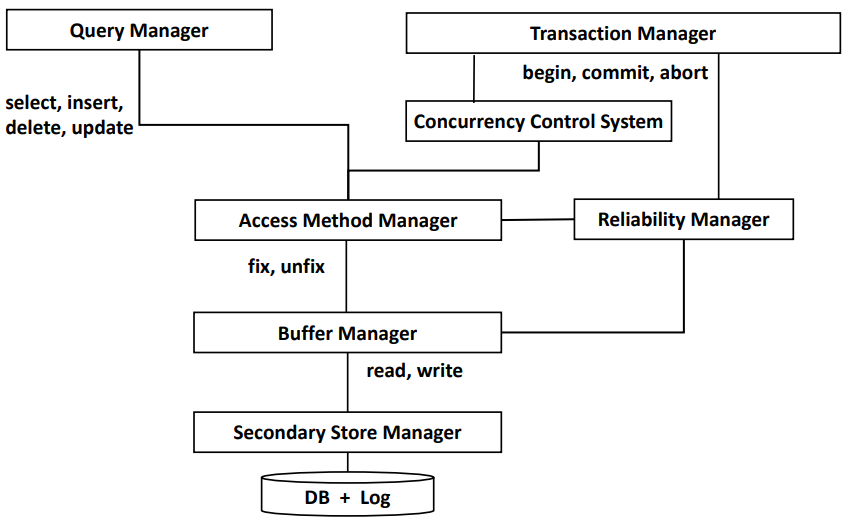
\includegraphics[width=0.5\linewidth]{images/architecture.png}
    \caption{DBMS architecture}
\end{figure}